\documentclass{elsart}

\usepackage{color}
\usepackage{cite}
\usepackage{url}
\usepackage{pgf,pgfarrows,pgfshade}
\usepackage{subfigure}
\usepackage{units}
\usepackage{amsmath}
\input{../cimis_acronyms}

\begin{document}
%
\begin{frontmatter}
\title{Title}  
%
\author[calspace]{Quinn~Hart}

\address[calspace]{CalSpace \\
University of California, Davis\\
Davis, CA, USA \\
{qjhart,carueda,slustin}@ucdavis.edu}

\end{frontmatter}                                

% This format puts a special copyright style on the first page
\thispagestyle{plain}

\begin{figure}
  \centering
  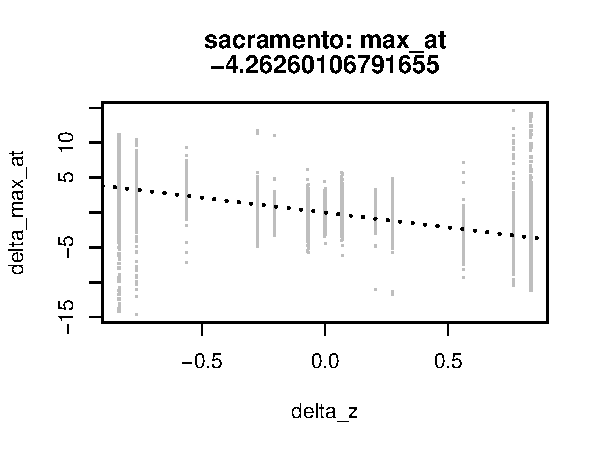
\includegraphics[width=0.3\textwidth]{lapse_rate/sacramento_max_at}
  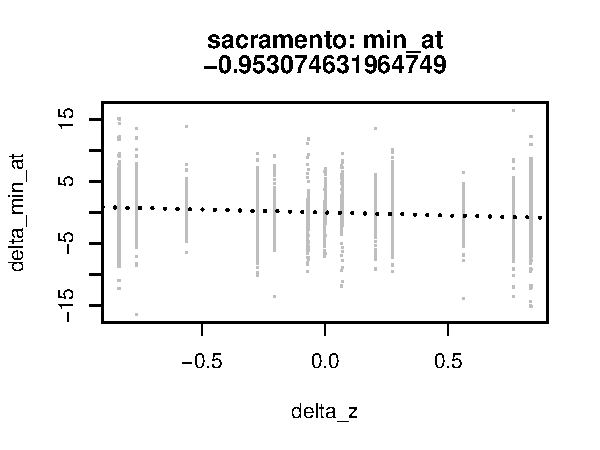
\includegraphics[width=0.3\textwidth]{lapse_rate/sacramento_min_at} 
  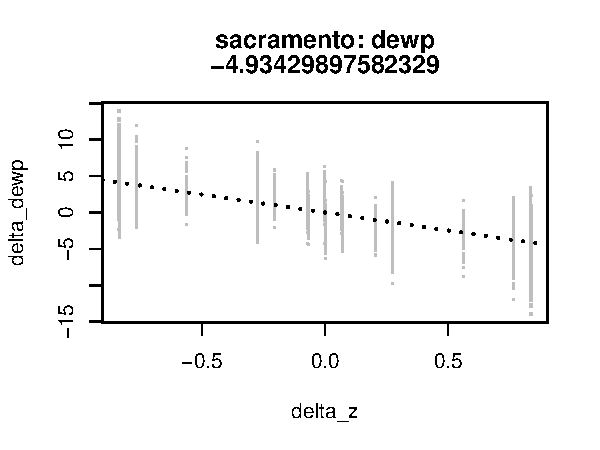
\includegraphics[width=0.3\textwidth]{lapse_rate/sacramento_dewp}

  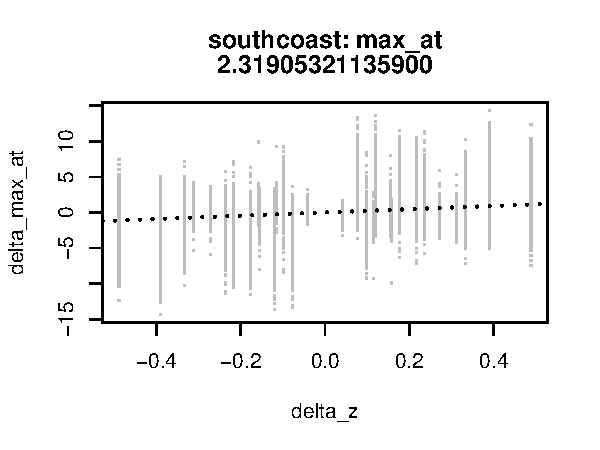
\includegraphics[width=0.3\textwidth]{lapse_rate/southcoast_max_at}
  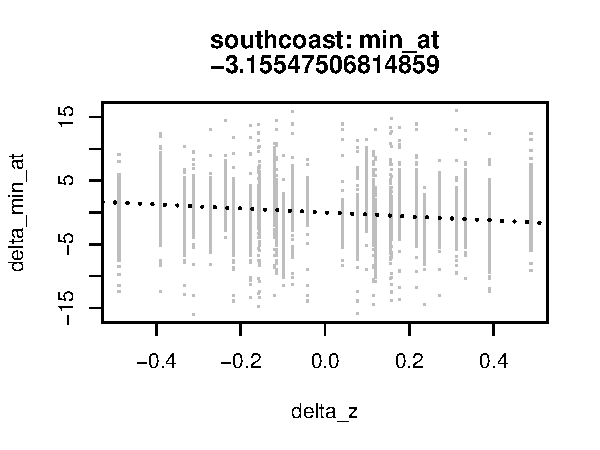
\includegraphics[width=0.3\textwidth]{lapse_rate/southcoast_min_at} 
  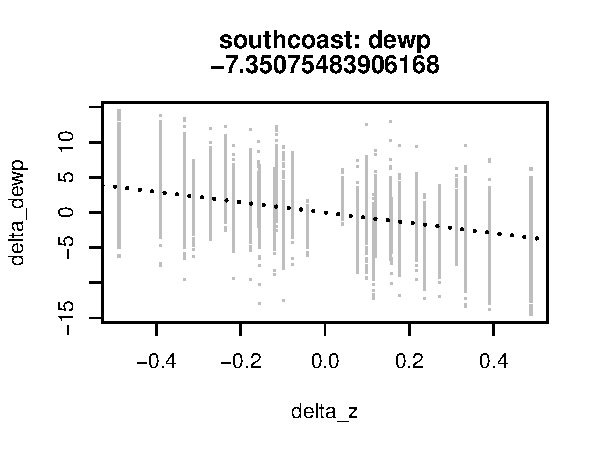
\includegraphics[width=0.3\textwidth]{lapse_rate/southcoast_dewp}

  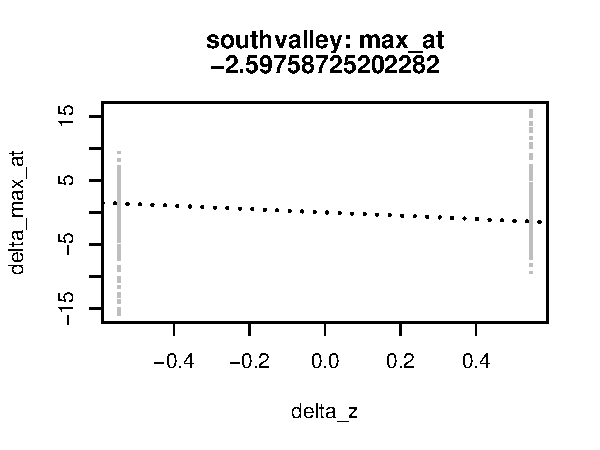
\includegraphics[width=0.3\textwidth]{lapse_rate/southvalley_max_at}
  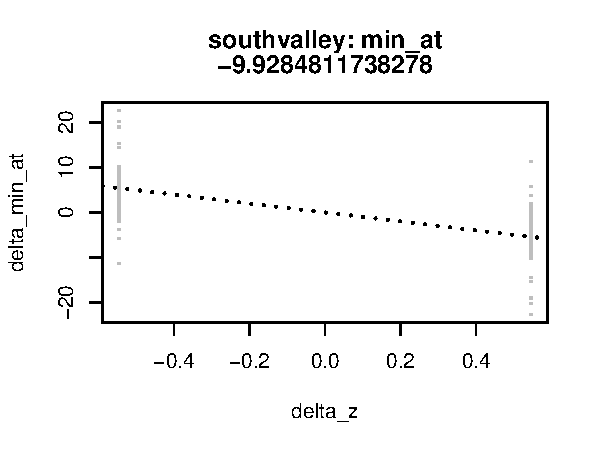
\includegraphics[width=0.3\textwidth]{lapse_rate/southvalley_min_at} 
  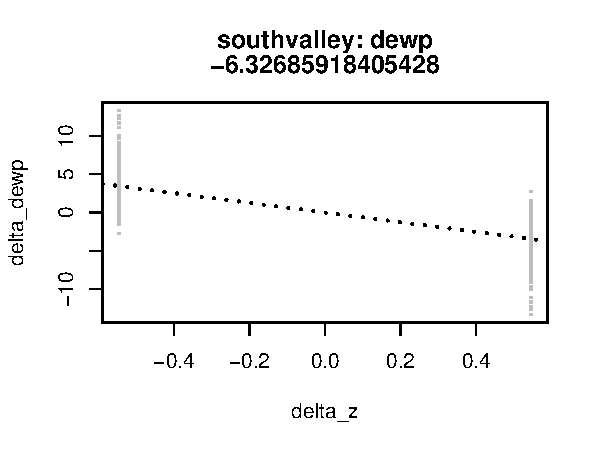
\includegraphics[width=0.3\textwidth]{lapse_rate/southvalley_dewp}

  \caption{Average lapse rates}
  \label{fig:lapse_rate}
\end{figure}

\begin{table}
  \centering
  \caption{Average monthly surface temperature lapse rate measurements $[\unitfrac{\ensuremath{^\circ}C}{km}]$ for various California transects.
  }
\begin{tabular}{c | c c c | c c c | c c c }
& \multicolumn{3}{c|}{South Coast} & \multicolumn{3}{c|}{South Valley} & \multicolumn{3}{c}{Sacramento} \\
\raisebox{1.5ex}{Month} & \acs{Tx} & \acs{Tn} & \acs{dewp} & \acs{Tx} & \acs{Tn}  &\acs{dewp} & \acs{Tx} & \acs{Tn} & \acs{dewp} \\ \hline \hline
\input{lapse_rate.tex}
\end{tabular}
\label{tab:lapse_rate}
\end{table}

\begin{figure}
  \centering
  \includegraphics[width=0.3\textwidth]{lapse_rate/sacramento_max_at_K}
  \includegraphics[width=0.3\textwidth]{lapse_rate/sacramento_min_at_K} 
  \includegraphics[width=0.3\textwidth]{lapse_rate/sacramento_dewp_K}

  \includegraphics[width=0.3\textwidth]{lapse_rate/southcoast_max_at_K}
  \includegraphics[width=0.3\textwidth]{lapse_rate/southcoast_min_at_K} 
  \includegraphics[width=0.3\textwidth]{lapse_rate/southcoast_dewp_K}

  \includegraphics[width=0.3\textwidth]{lapse_rate/southvalley_max_at_K}
  \includegraphics[width=0.3\textwidth]{lapse_rate/southvalley_min_at_K} 
  \includegraphics[width=0.3\textwidth]{lapse_rate/southvalley_dewp_K}

  \caption{Average lapse rates (Clear sky $\acs{K} > 0.85$}
  \label{fig:lapse_rate}
\end{figure}

\begin{table}
  \centering
  \caption{Average monthly surface temperature lapse rate measurements $[\unitfrac{\ensuremath{^\circ}C}{km}]$ for various California transects.  Clear Skies only, $\acs{K} > 0.85$
  }
\begin{tabular}{c | c c c | c c c | c c c }
& \multicolumn{3}{c|}{South Coast} & \multicolumn{3}{c|}{South Valley} & \multicolumn{3}{c}{Sacramento} \\
\raisebox{1.5ex}{Month} & \acs{Tx} & \acs{Tn} & \acs{dewp} & \acs{Tx} & \acs{Tn}  &\acs{dewp} & \acs{Tx} & \acs{Tn} & \acs{dewp} \\ \hline \hline
Jan& -3.34& -3.81& -9.44& 3.25& -7.29& -7.66& 0.20& -1.93& -4.93\\
Feb& -3.13& -3.68& -10.22& -3.93& -7.50& -6.48& -4.50& -2.29& -5.62\\
Mar& 0.46& -3.94& -7.58& -4.73& -10.39& -6.14& -5.54& -2.49& -5.49\\
Apr& -0.46& -3.97& -6.42& -4.67& -10.18& -5.59& -6.50& -2.84& -3.83\\
May& 4.15& -3.09& -6.52& -3.79& -10.69& -5.65& -6.48& -2.43& -3.58\\
Jun& 6.63& -5.31& -3.76& -3.63& -12.83& -5.09& -5.47& -1.27& -3.33\\
Jul& 10.36& -2.38& -4.63& -2.91& -13.02& -6.46& -3.53& 2.67& -4.94\\
Aug& 9.99& -2.02& -6.04& -3.23& -12.51& -5.45& -3.09& 2.38& -6.50\\
Sep& 6.22& -0.80& -7.30& -3.17& -11.39& -5.39& -4.08& 0.81& -6.97\\
Oct& 1.56& -1.68& -5.74& -3.53& -8.34& -6.69& -4.68& -0.33& -5.27\\
Nov& -2.20& -3.64& -9.45& -0.94& -6.87& -8.38& -2.64& -0.55& -4.56\\
Dec& -3.05& -3.23& -11.06& 1.62& -5.71& -8.43& -2.33& -1.74& -4.28\\

\end{tabular}
\label{tab:lapse_rate}
\end{table}

\end{document}
